\documentclass{amsart}
\usepackage{amsmath, amssymb}
\usepackage{mathpartir}
\usepackage{listings}
\usepackage{fancyvrb}
\usepackage{color}
\usepackage{bussproofs}
\usepackage{graphicx}
\usepackage{pgf, tikz}
\usetikzlibrary{arrows, automata}

\fvset{%
  fontsize=\small,
  numbers=left
}

\makeatletter
\renewcommand{\Pr}[1]{\text{\textbf{Pr}}\left(#1\right)}
\renewcommand\subsection{\@startsection{subsection}{2}%
  \z@{-.5\linespacing\@plus-.7\linespacing}{.5\linespacing}%
  {\normalfont\scshape}}
\renewcommand\subsubsection{\@startsection{subsubsection}{3}%
  \z@{.5\linespacing\@plus.7\linespacing}{-.5em}%
  {\normalfont\scshape}}
\makeatother

\title{Paper section: Urbanization in Shanghai}
\author{Evan Bergeron\\
\today
}

\begin{document}
\maketitle

\begin{figure}[h]
\centering
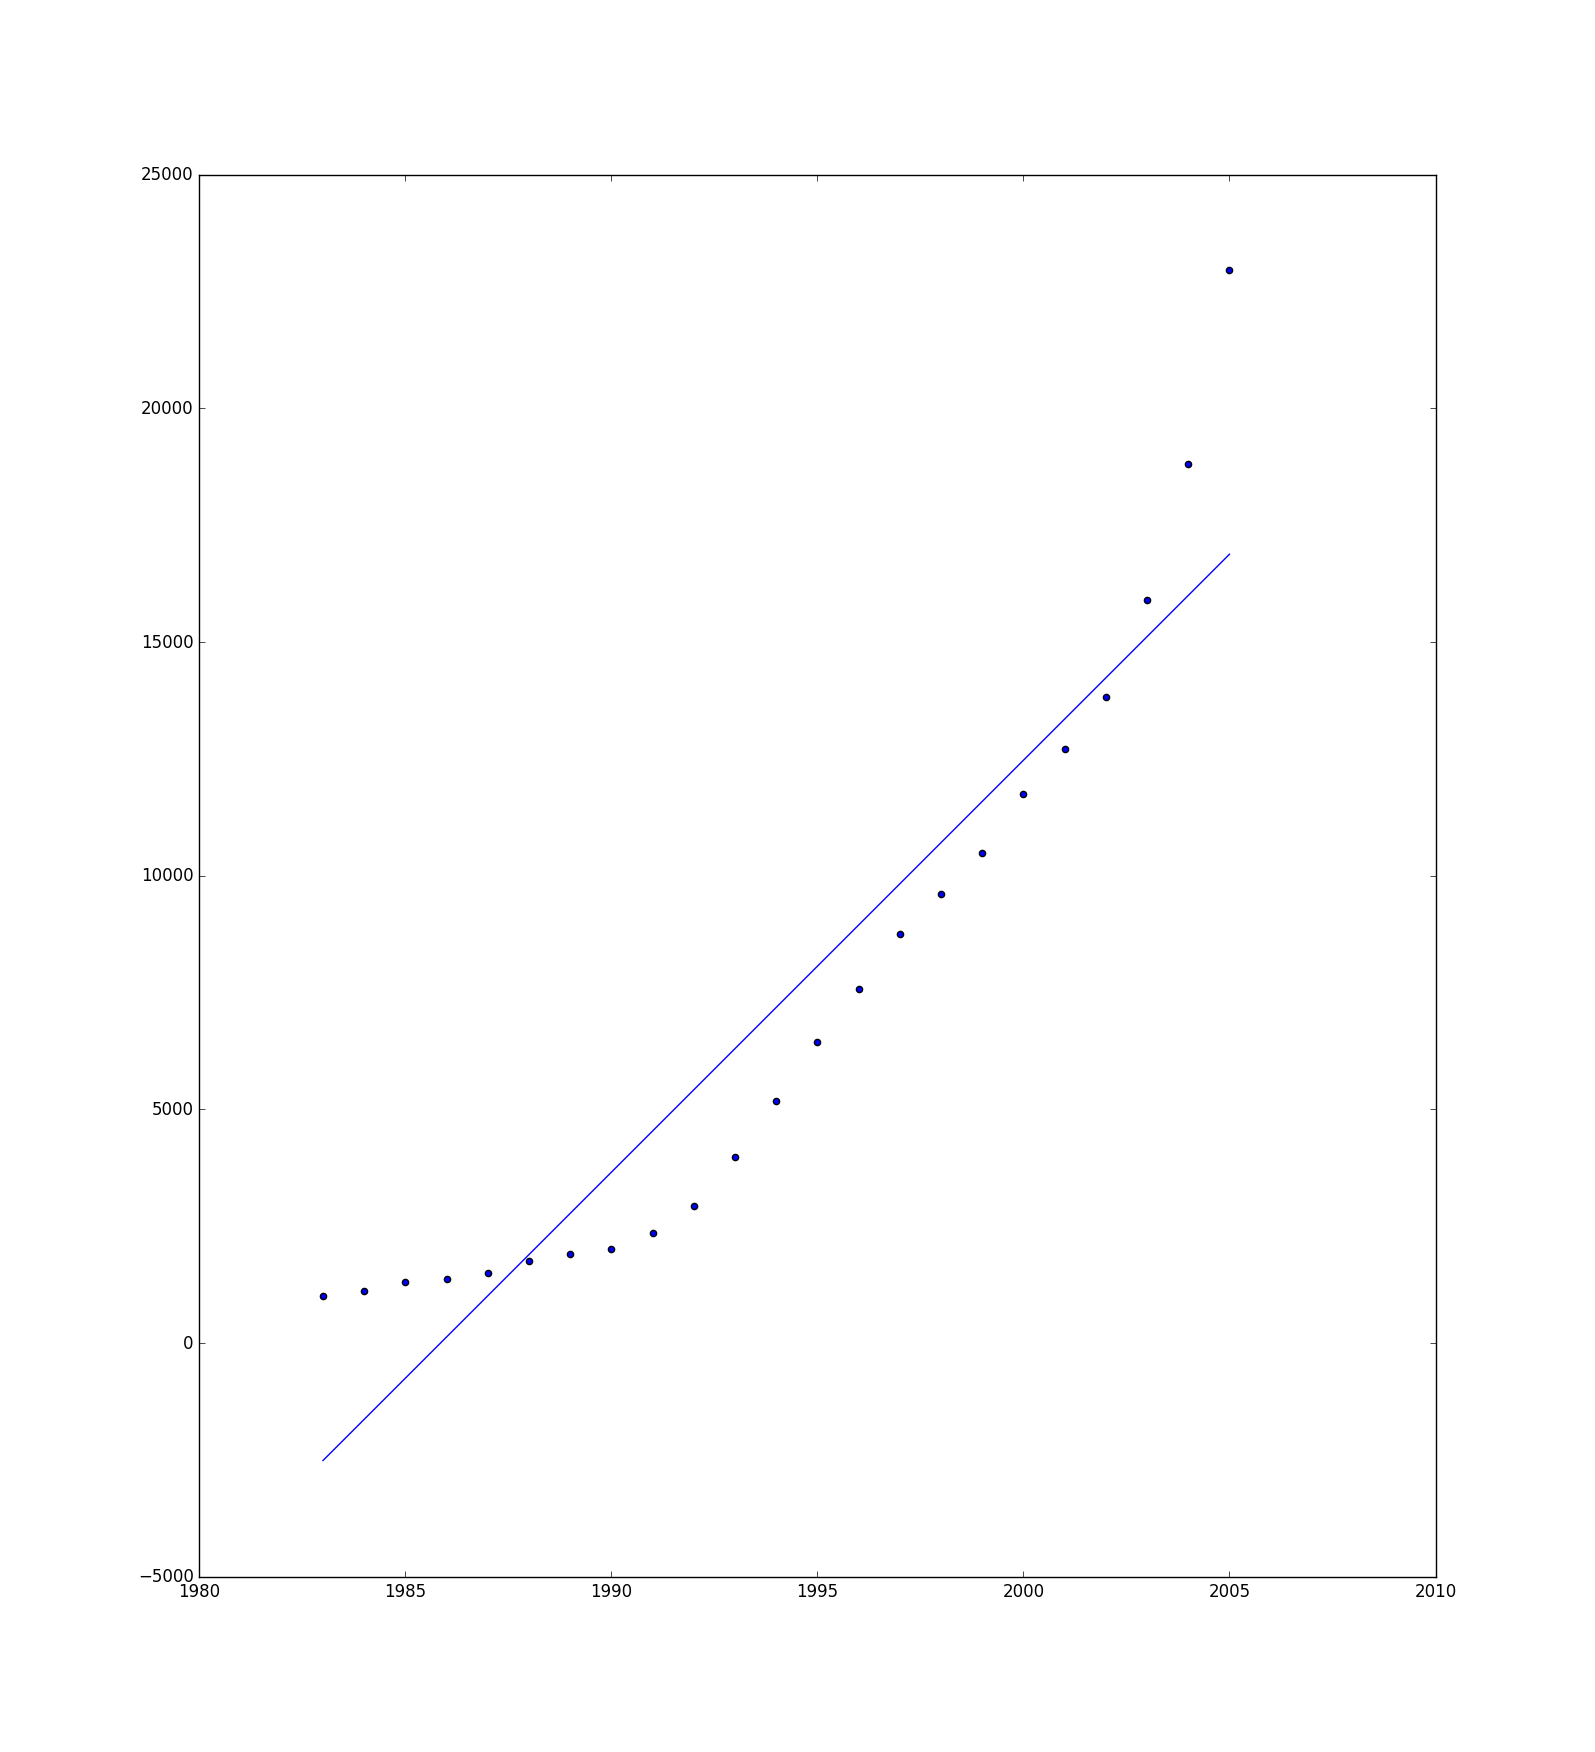
\includegraphics[width=0.5\textwidth]{img/growth_gdp}
\caption{GDP growth over time}
\end{figure}

\begin{figure}[h]
\centering
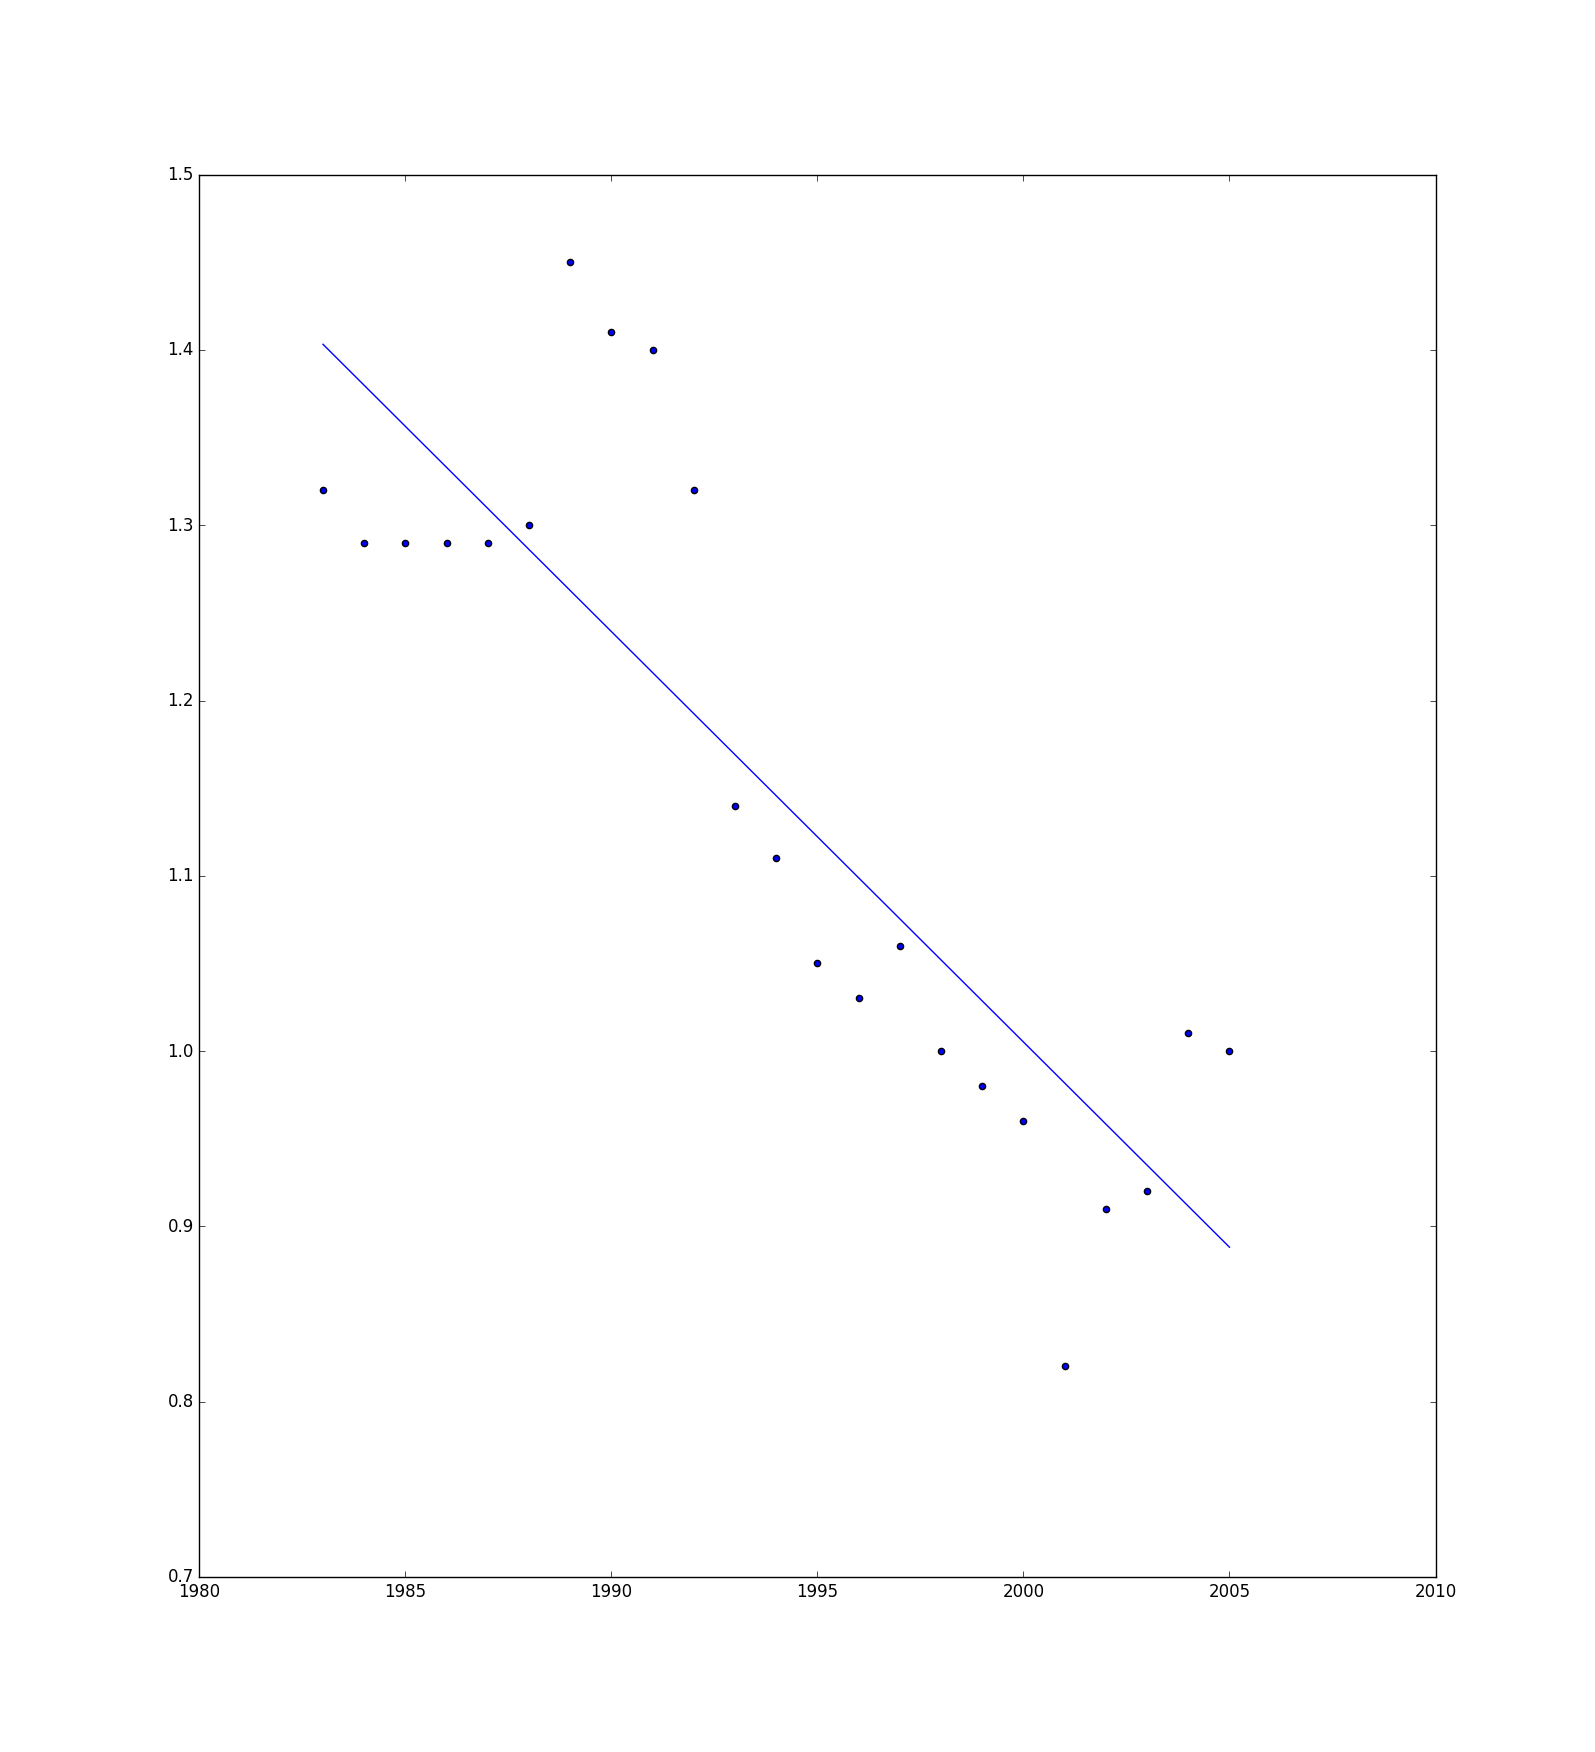
\includegraphics[width=0.5\textwidth]{img/air_quality}
\caption{Air quality over time}
\end{figure}

\begin{figure}[h]
\centering
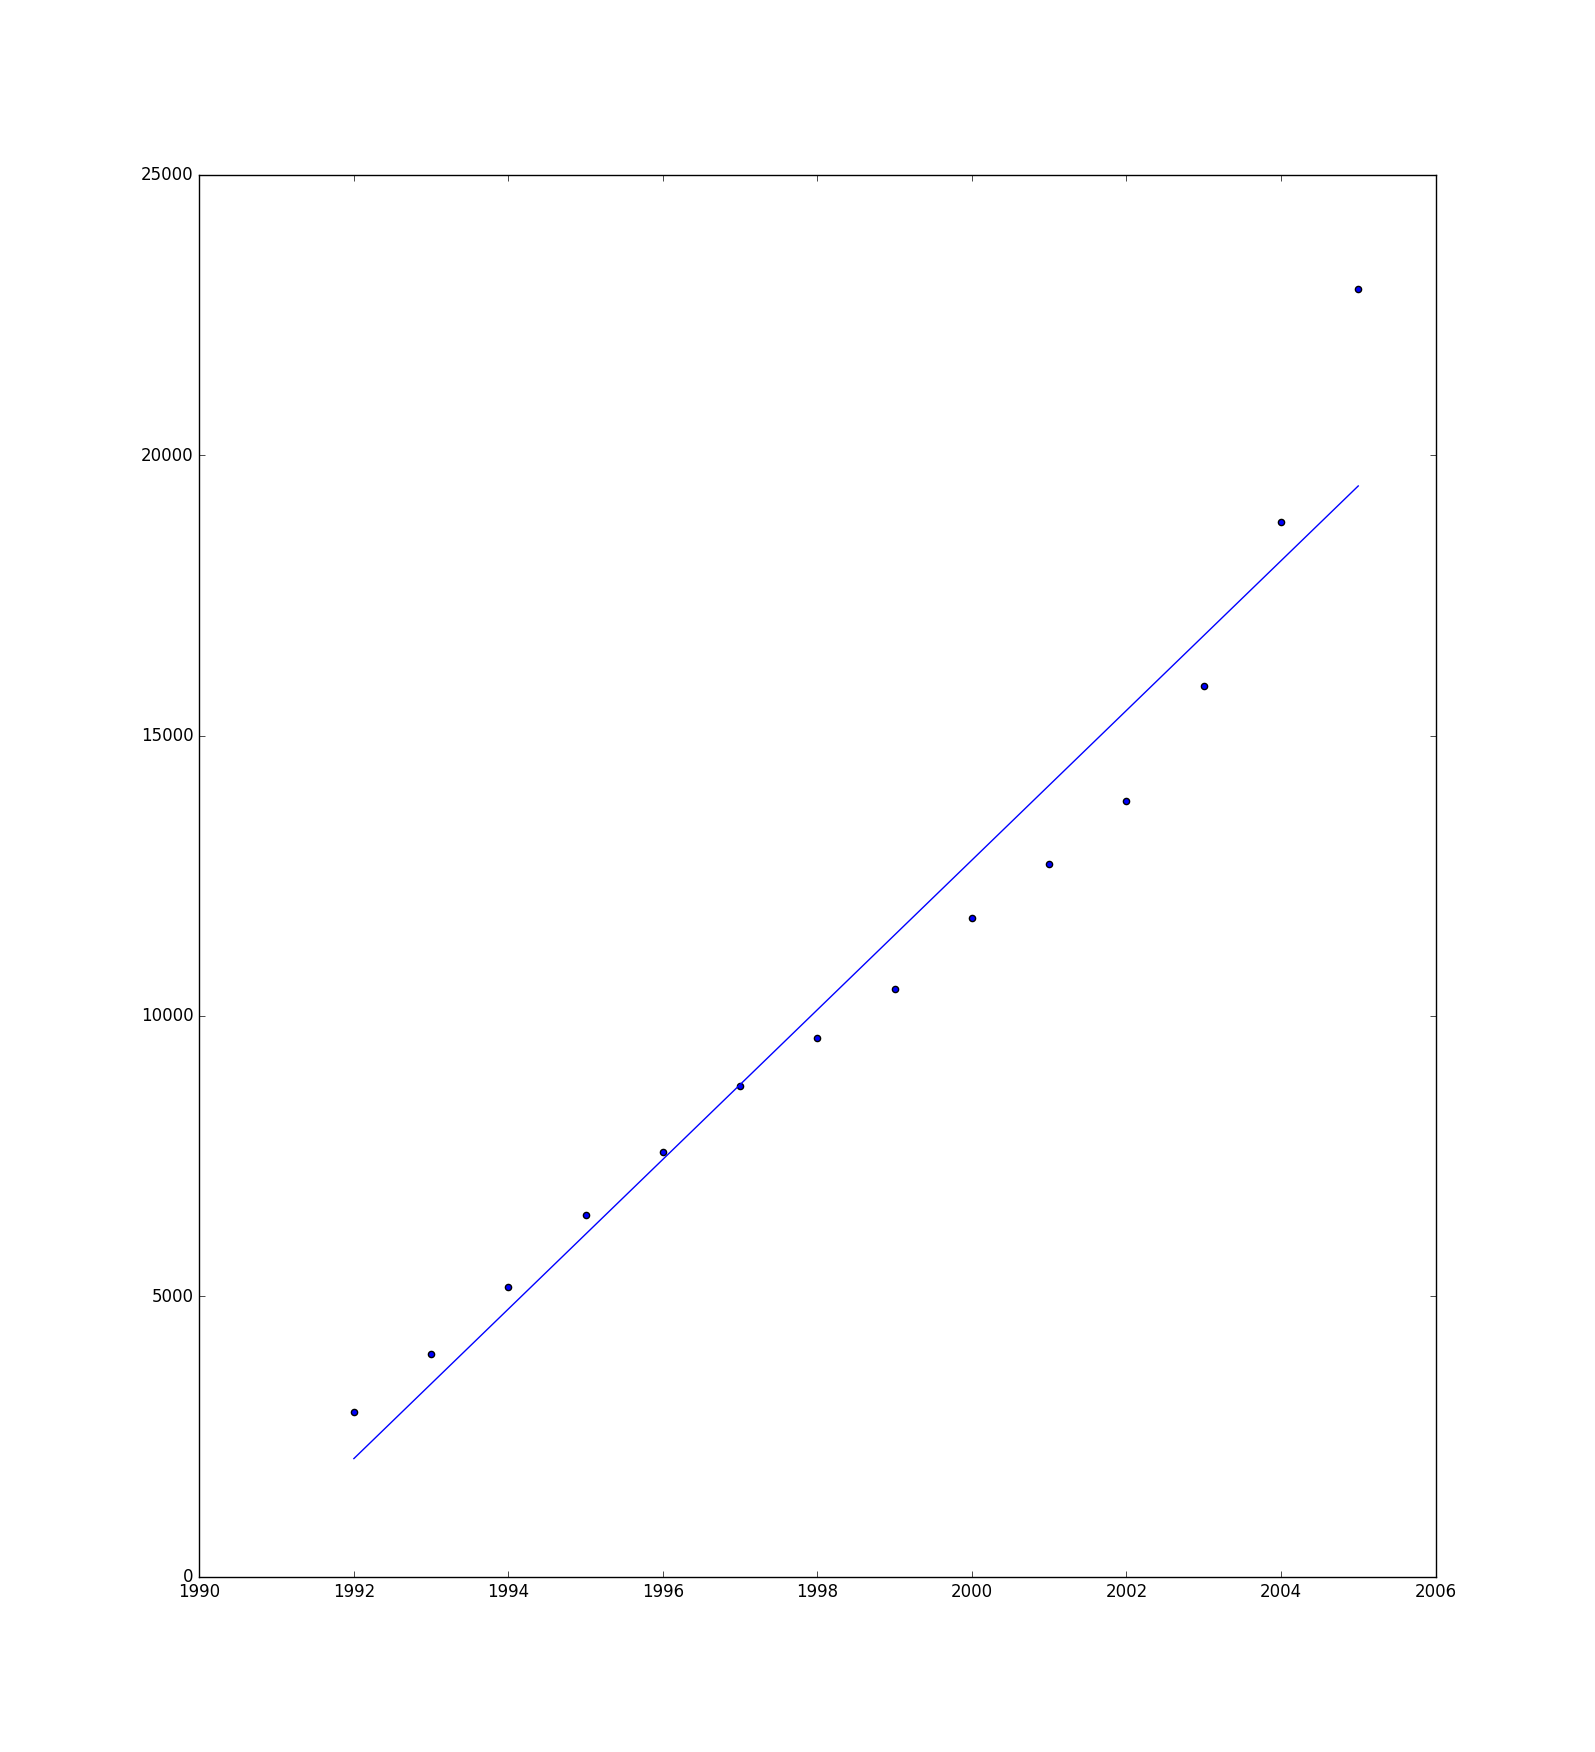
\includegraphics[width=0.5\textwidth]{img/growth_gdp_1991}
\caption{GDP growth since 1991}
\end{figure}

\begin{figure}[h]
\centering
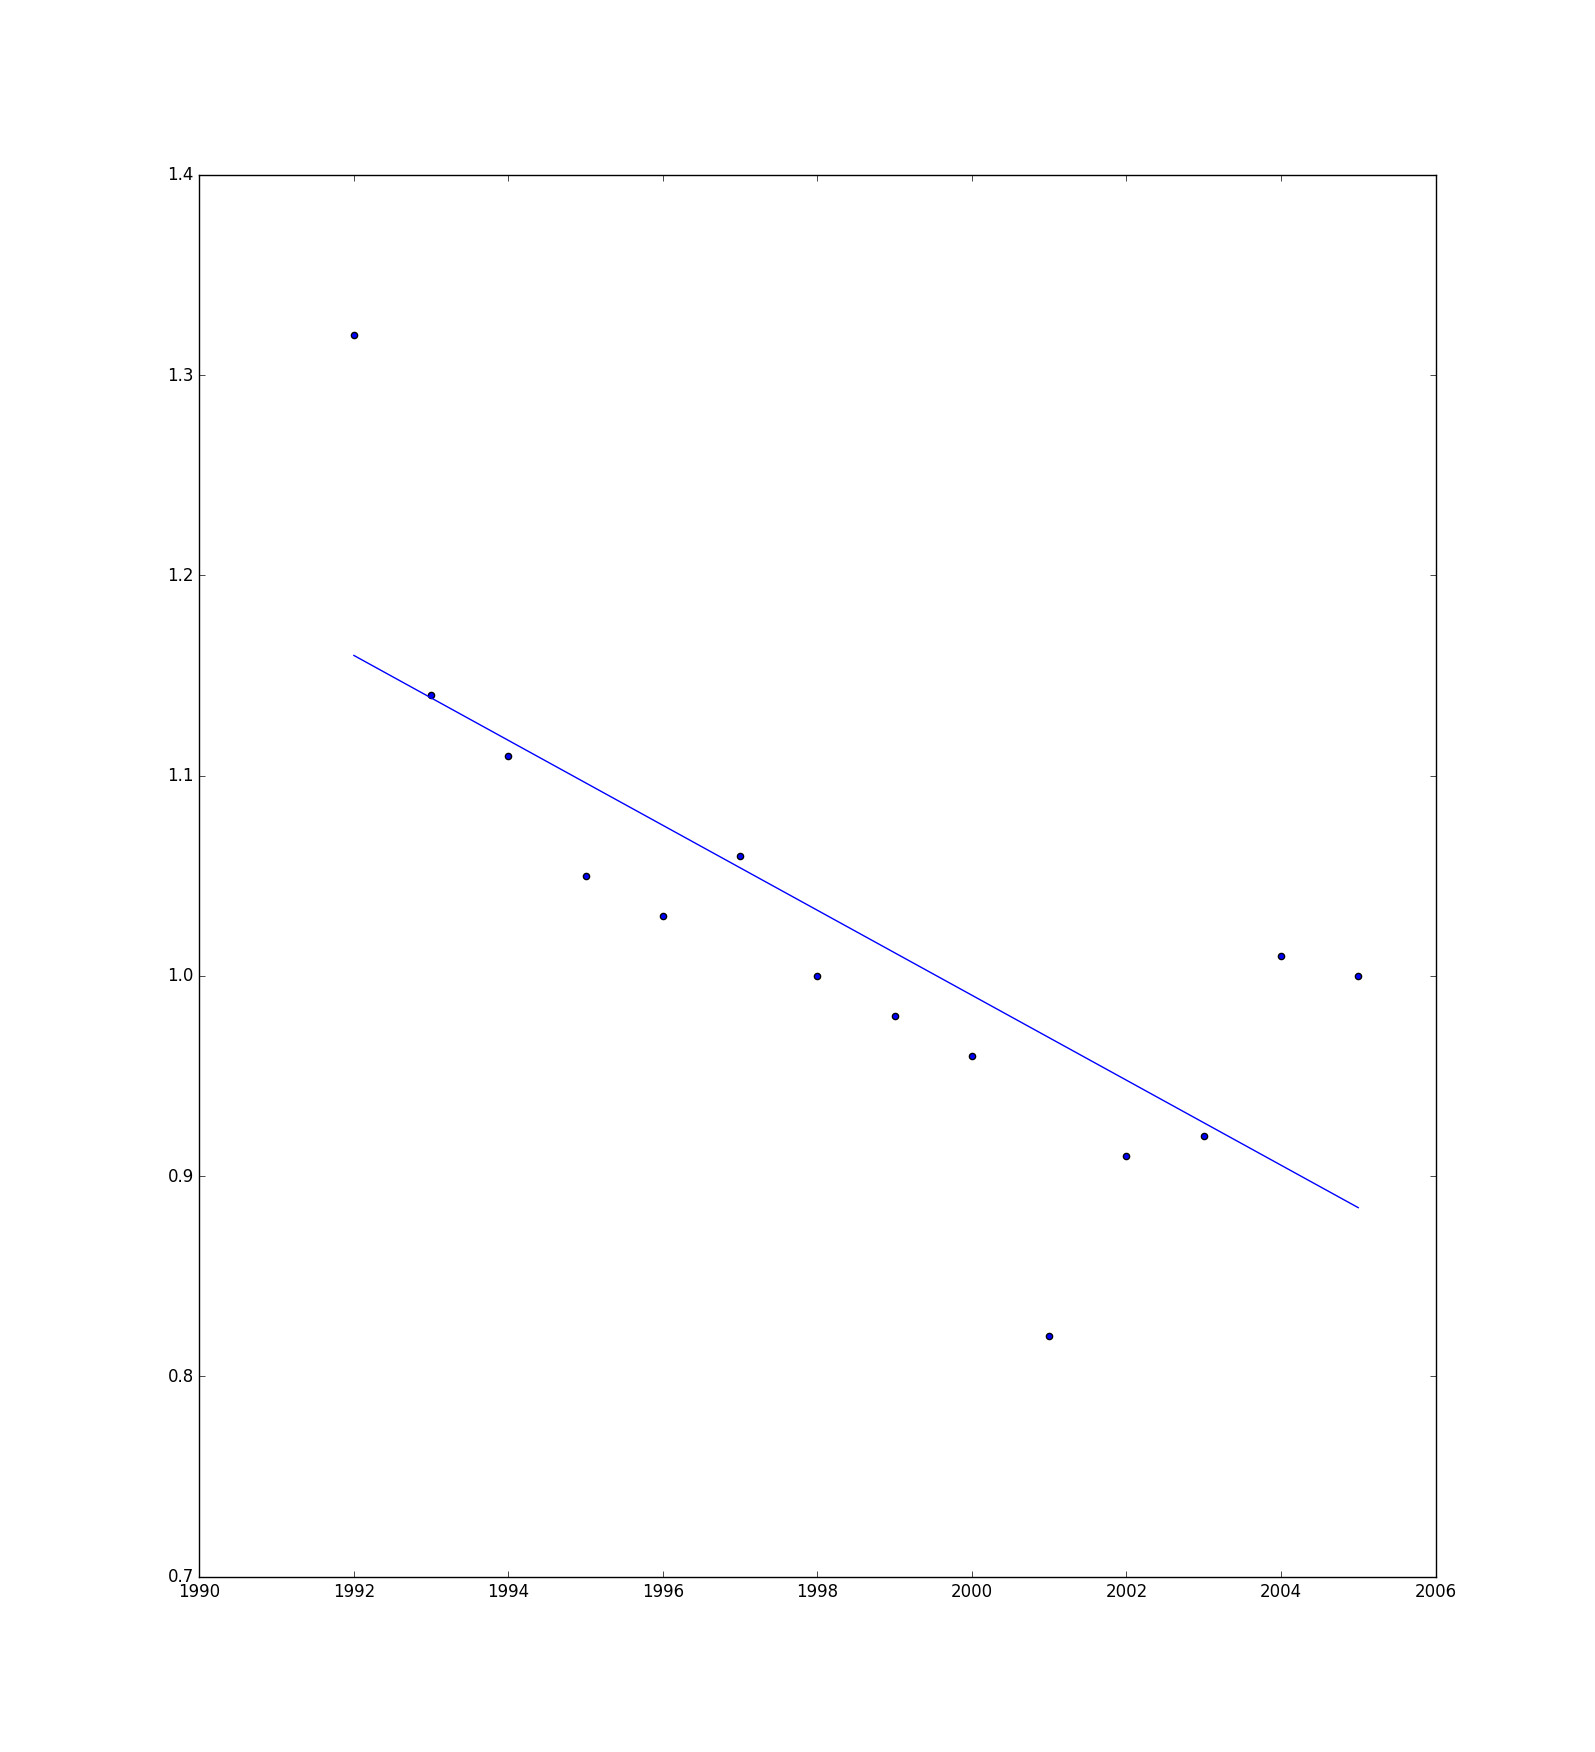
\includegraphics[width=0.5\textwidth]{img/air_quality_1991}
\caption{Air quality since 1991}
\end{figure}


\end{document}
